% =============================================================================
\section{Panorama: qué es x500\_retos}
% =============================================================================

\begin{frame}{Idea central}
  \begin{columns}[c]
    \column{0.5\textwidth}
    \begin{idea}
      Ya saben mover un dron con ROS 2 y PX4 (\cmd{px4\_examples}). Ahora toca
      \textbf{resolver misiones del mundo real}, cada una en su propio mundo de
      Gazebo, y de la más fácil a la más difícil.
    \end{idea}
    \vspace{0.5em}
    \small Todo es \textbf{100\% simulación}: se vale chocar, perder el control,
    vaciar la batería\ldots{} y volver a empezar.
    \column{0.48\textwidth}
    \begin{tikzpicture}[node distance=0.55cm, every node/.style={font=\scriptsize}]
      \node[draw=azul,fill=azulclaro,rounded corners,minimum width=3.6cm] (ex) {px4\_examples: las piezas};
      \node[draw=azul,fill=azulclaro,rounded corners,minimum width=3.6cm,below=of ex] (n1) {Nivel 1: moverse bien};
      \node[draw=azul,fill=azulclaro,rounded corners,minimum width=3.6cm,below=of n1] (n2) {Nivel 2: decidir solo};
      \node[draw=azul,fill=azulclaro,rounded corners,minimum width=3.6cm,below=of n2] (n3) {Nivel 3: ver con cámara};
      \draw[-{Stealth},thick,azul] (ex) -- (n1);
      \draw[-{Stealth},thick,azul] (n1) -- (n2);
      \draw[-{Stealth},thick,azul] (n2) -- (n3);
    \end{tikzpicture}
  \end{columns}
\end{frame}

\begin{frame}{Las siete misiones}
  \centering\small
  \begin{tabular}{clllp{4.6cm}}
    \toprule
    \# & Misión & Mundo & Nodo & Qué se aprende \\
    \midrule
    1 & Estrella del show & \cmd{plaza\_show} & \cmd{estrella\_show} & Generar waypoints con una fórmula \\
    2 & Inspección de un pilar & \cmd{puente\_rio} & \cmd{inspeccion\_pilar} & Hélice con feedforward y yaw al centro \\
    3 & Entrega a domicilio & \cmd{barrio\_entrega} & \cmd{entrega\_domicilio} & Misión por etapas con comandos de PX4 \\
    \midrule
    4 & Geocerca del concierto & \cmd{plaza\_concierto} & \cmd{guardian\_geocerca} & Un nodo que vigila y predice el frenado \\
    5 & Cruzar una cueva & \cmd{cueva} & \cmd{cruzar\_cueva} & Control reactivo con lidar 2D \\
    \midrule
    6 & Caza del objetivo & \cmd{zona\_bodegas} & \cmd{caza\_objetivo} & Cámara, ArUco y seguir algo que se mueve \\
    7 & Estación de carga & \cmd{base\_carga} & \cmd{estacion\_carga} & Batería y aterrizaje de precisión \\
    \bottomrule
  \end{tabular}
  \vspace{0.6em}

  \footnotesize Nivel 3 además tiene \cmd{detector\_aruco}: los ``ojos'' que comparten las misiones 6 y 7.
\end{frame}

\begin{frame}{Los mundos (1/2)}
  \begin{columns}[t]
    \column{0.33\textwidth}\centering
    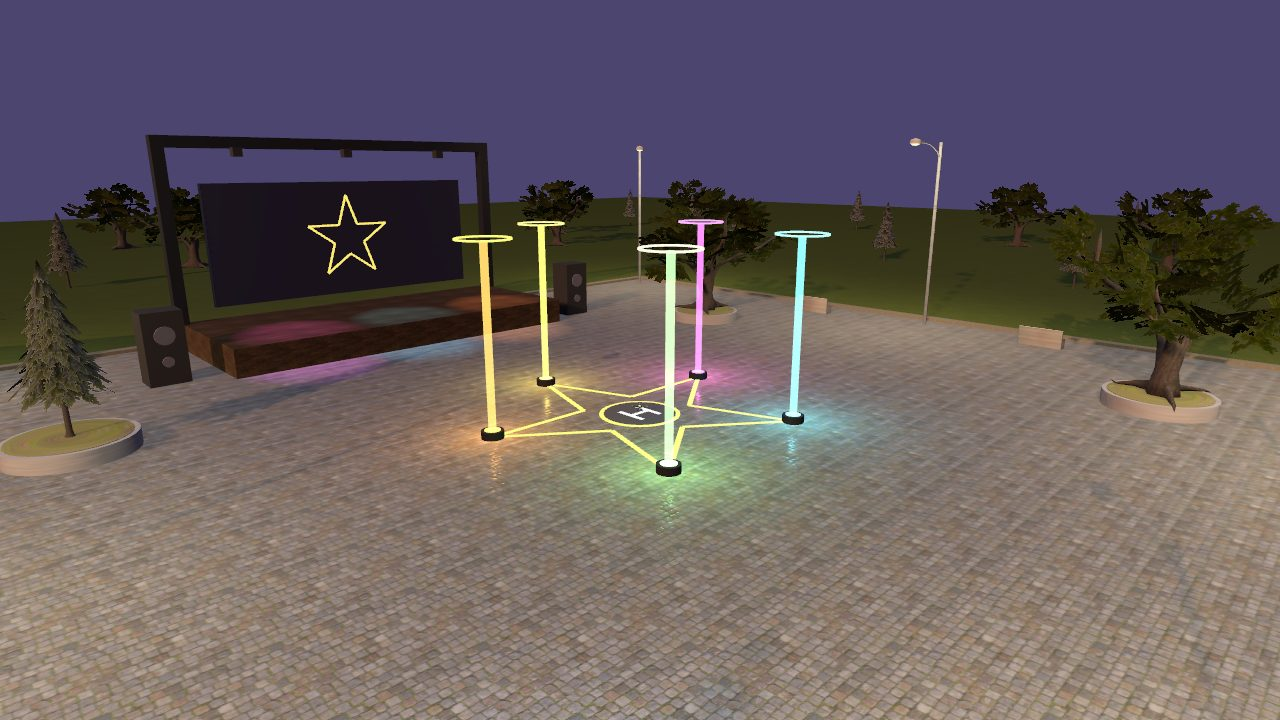
\includegraphics[width=\linewidth]{plaza_show_estrella}\\
    {\scriptsize \cmd{plaza\_show}: la estrella dorada y las 5 balizas con aros a 6 m}
    \column{0.33\textwidth}\centering
    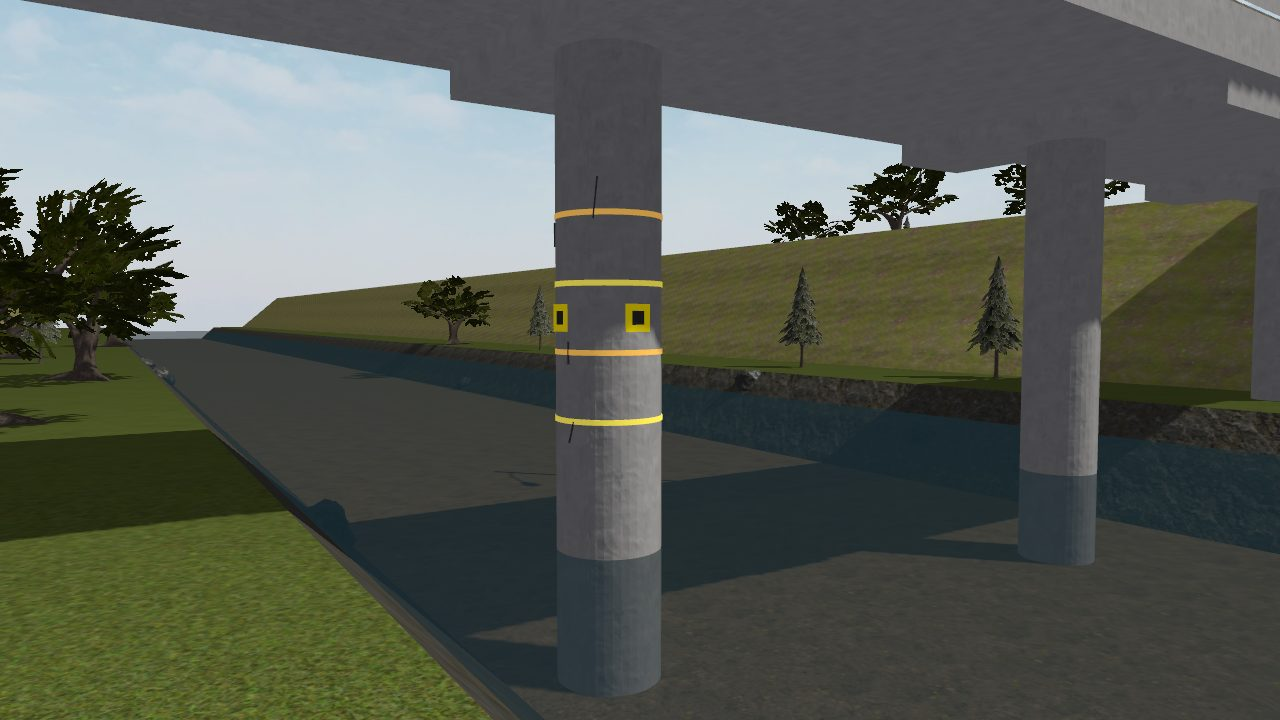
\includegraphics[width=\linewidth]{puente_rio_pilar}\\
    {\scriptsize \cmd{puente\_rio}: el pilar con bandas a 1, 2, 3 y 4 m}
    \column{0.33\textwidth}\centering
    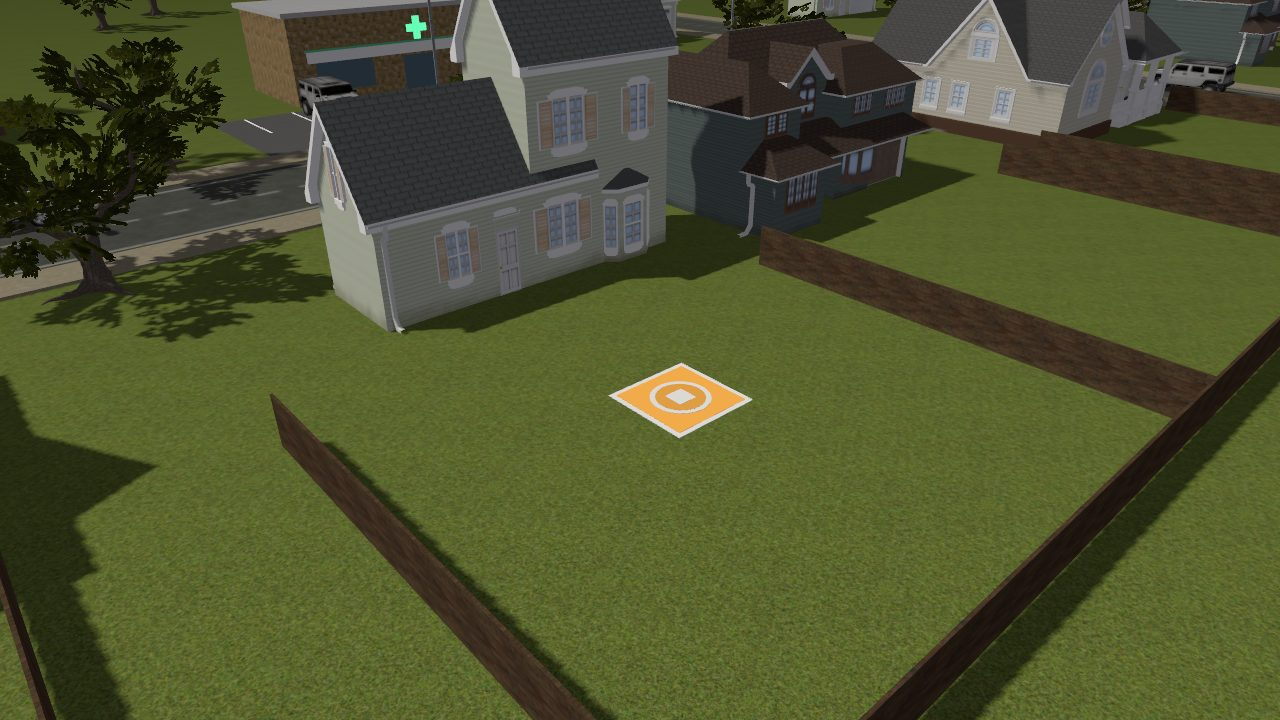
\includegraphics[width=\linewidth]{barrio_entrega_patio}\\
    {\scriptsize \cmd{barrio\_entrega}: la plataforma naranja en el patio, a 39.4 m}
  \end{columns}
\end{frame}

\begin{frame}{Los mundos (2/2)}
  \begin{columns}[t]
    \column{0.25\textwidth}\centering
    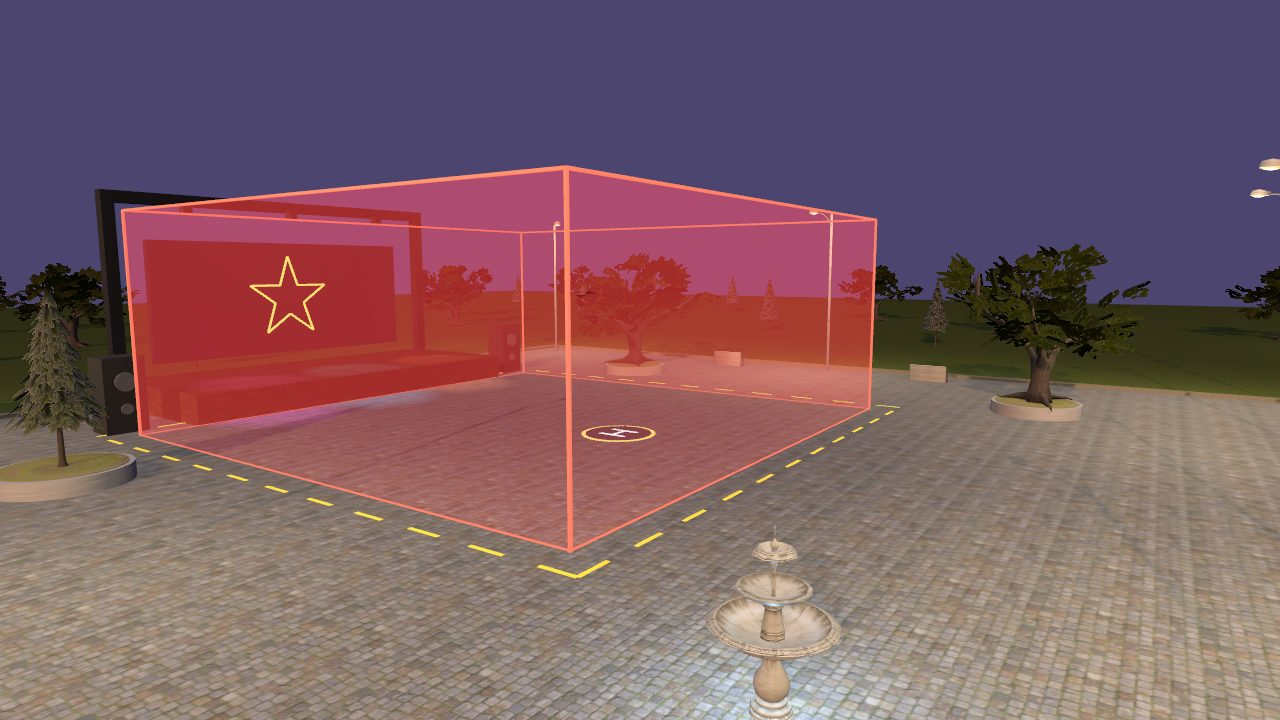
\includegraphics[width=\linewidth]{plaza_concierto}\\
    {\scriptsize \cmd{plaza\_concierto}: la geocerca roja}
    \column{0.25\textwidth}\centering
    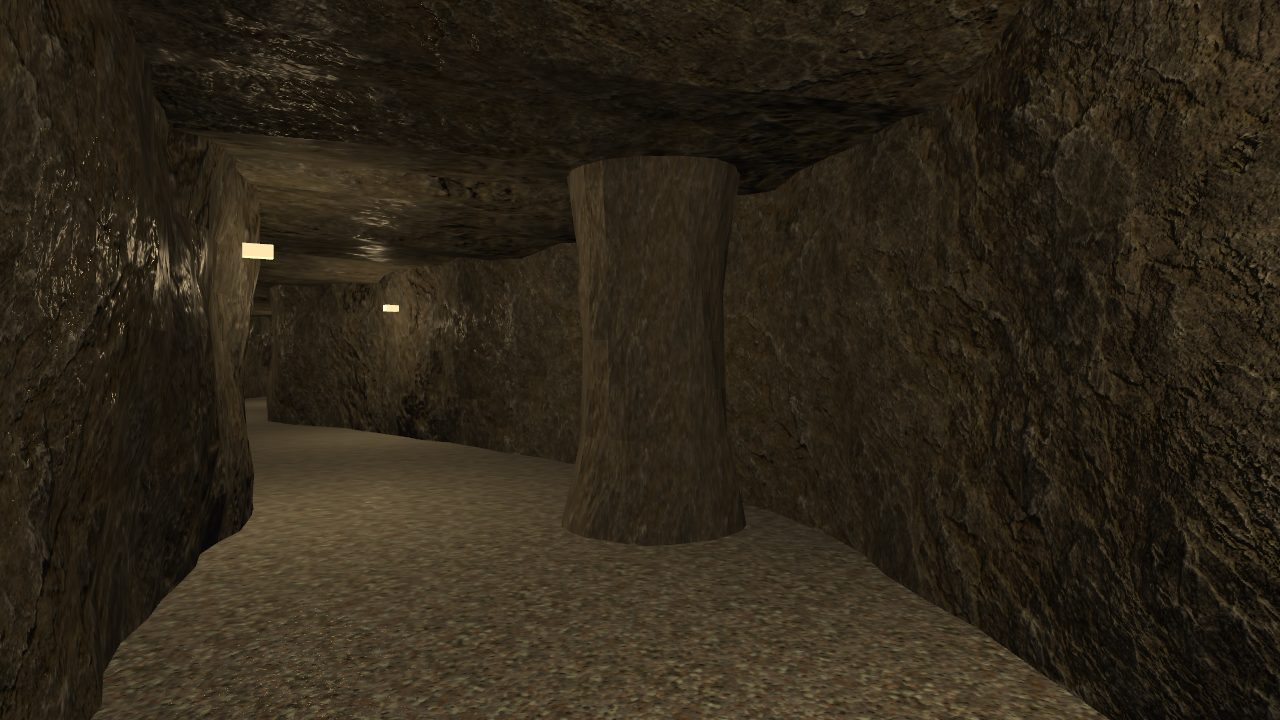
\includegraphics[width=\linewidth]{cueva_columna}\\
    {\scriptsize \cmd{cueva}: el túnel y la columna}
    \column{0.25\textwidth}\centering
    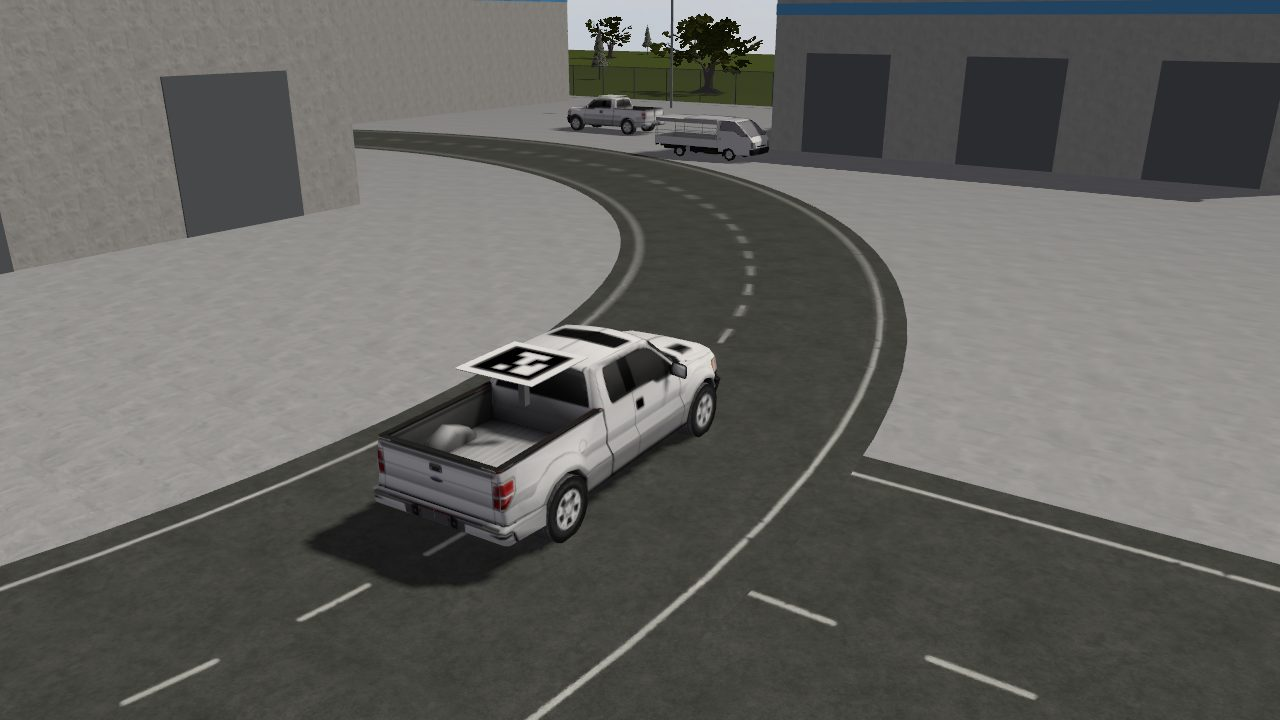
\includegraphics[width=\linewidth]{zona_bodegas_camioneta}\\
    {\scriptsize \cmd{zona\_bodegas}: la camioneta del ArUco 7}
    \column{0.25\textwidth}\centering
    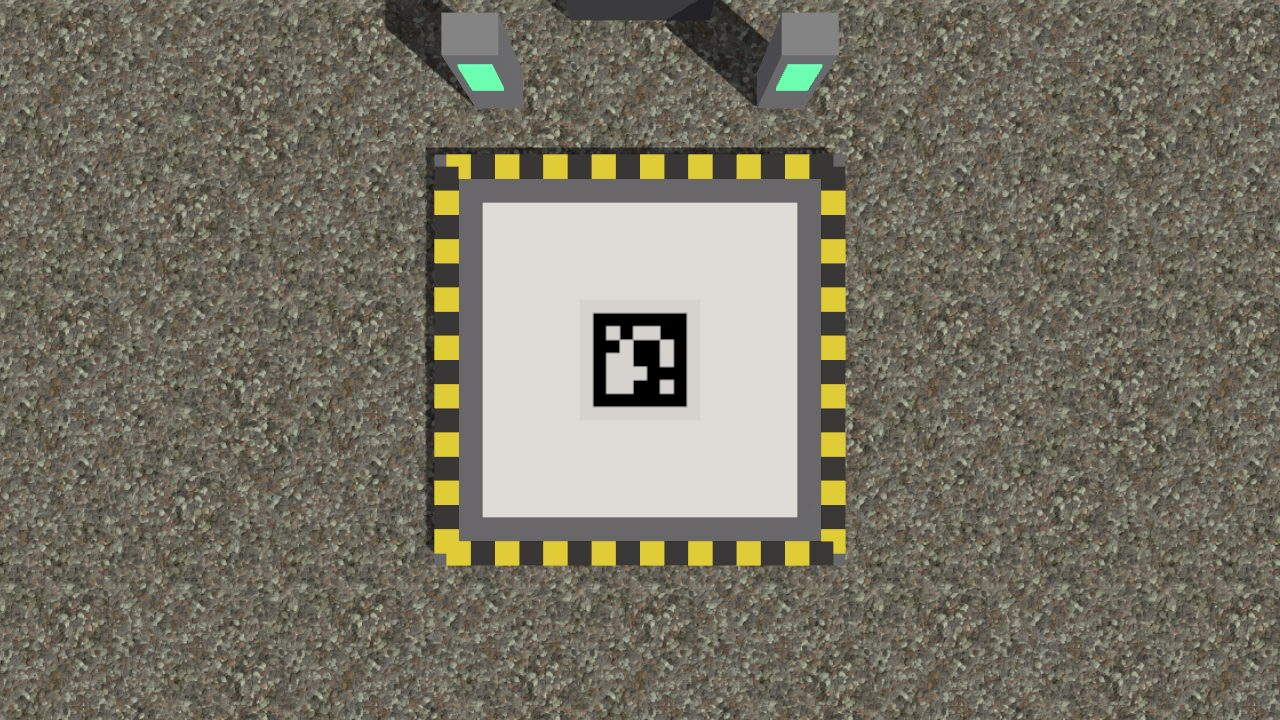
\includegraphics[width=\linewidth]{base_carga_estacion}\\
    {\scriptsize \cmd{base\_carga}: la estación con el ArUco 42}
  \end{columns}
\end{frame}

\begin{frame}{Cómo está hecho un reto}
  \begin{columns}[c]
    \column{0.52\textwidth}\small
    Cada misión es \textbf{un nodo que ya funciona}:
    \begin{itemize}
      \item La máquina de estados, los parámetros, el log y la medición del
        resultado \textbf{ya están hechos}.
      \item Lo que pide el reto está marcado con \cmd{// TODO} y pistas.
      \item Mientras no lo resuelvas, el nodo vuela de forma \textbf{segura}:
        despega, avisa qué falta, regresa y aterriza.
      \item Al final, el propio nodo te dice \textbf{``Misión cumplida''} o
        \textbf{``Misión NO cumplida''}.
    \end{itemize}
    \column{0.45\textwidth}
    \begin{terminal}{ros2 run x500\_retos estrella\_show}
OFFBOARD activo, subiendo a 6.0 m\\
vertices() regresó una lista vacía:\\
\ \ falta el TODO. Aterrizando\\
Aterrizado. Qué tan cerca pasó...\\
Misión NO cumplida
    \end{terminal}
  \end{columns}
\end{frame}

\begin{frame}{Qué se entrega por misión}
  \begin{enumerate}
    \item El nodo resuelto (los \cmd{TODO}), compilando \textbf{sin warnings}.
    \item Una corrida donde el nodo diga \textbf{``Misión cumplida''} (tres corridas seguidas para la rúbrica).
    \item Un README de 5 líneas: qué hace, cómo se corre, qué parámetros tiene.
    \item Un video corto de Gazebo + QGroundControl.
  \end{enumerate}
  \vspace{0.5em}
  \begin{idea}
    \textbf{Regla de oro:} nada de números mágicos. Alturas, radios, velocidades y
    tiempos van como parámetros (\cmd{--ros-args -p radio:=4.0}), igual que en
    \cmd{orbit\_mission}.
  \end{idea}
\end{frame}

\begin{frame}{Dónde vive cada cosa}
  \begin{columns}[c]
    \column{0.5\textwidth}
    \begin{tikzpicture}[every node/.style={font=\scriptsize\ttfamily,anchor=west}]
      \node at (0,0)    {src/x500\_retos/};
      \node at (0.3,-0.4) {include/x500\_retos/ \textrm{\color{gris}(px4\_link, aruco\_tools)}};
      \node at (0.3,-0.8) {src/ \textrm{\color{gris}(un .cpp por misión)}};
      \node at (0.3,-1.2) {msg/ \textrm{\color{gris}(Aruco, ArucoArray)}};
      \node at (0.3,-1.6) {launch/ \textrm{\color{gris}(cueva, caza, estacion)}};
      \node at (0.3,-2.0) {worlds/ \textrm{\color{gris}(los 7 mundos + spawn.yaml)}};
      \node at (0.3,-2.4) {models/ \textrm{\color{gris}(Fuel, texturas, x500\_cam\_abajo)}};
      \node at (0.3,-2.8) {tools/ \textrm{\color{gris}(build\_worlds, make\_aruco, render)}};
      \node at (0.3,-3.2) {docs/ \textrm{\color{gris}(capturas y esta presentación)}};
    \end{tikzpicture}
    \column{0.48\textwidth}\small
    \begin{itemize}
      \item \cmd{src/}: \textbf{aquí trabajan}.
      \item \cmd{include/}: lo que comparten todas las misiones; léanlo, no hace falta cambiarlo.
      \item \cmd{worlds/} se \textbf{genera} con \cmd{tools/build\_worlds.py}: cambios a mano se pierden.
      \item \cmd{CREDITS.md}: licencias de los modelos y texturas.
    \end{itemize}
  \end{columns}
\end{frame}

\begin{frame}{De dónde viene cada misión}
  \centering
  \begin{tikzpicture}[x=1cm,y=0.75cm,every node/.style={font=\scriptsize}]
    \tikzset{ex/.style={draw=gris,fill=gray!10,rounded corners,minimum width=2.5cm,minimum height=0.5cm},
             mi/.style={draw=azul,fill=azulclaro,rounded corners,minimum width=2.6cm,minimum height=0.5cm}}
    \node[ex] (sq) at (0,4) {square\_mission};
    \node[ex] (or) at (0,3) {orbit\_mission};
    \node[ex] (f8) at (0,2) {figure\_eight};
    \node[ex] (go) at (0,1) {goto\_mission};
    \node[ex] (rh) at (0,0) {return\_home / set\_home};
    \node[ex] (fm) at (0,-1) {flight\_mode\_monitor};
    \node[ex] (vc) at (0,-2) {velocity\_control};
    \node[ex] (bm) at (0,-3) {battery\_monitor};
    \node[mi] (m1) at (6,4) {1 estrella\_show};
    \node[mi] (m2) at (6,2.5) {2 inspeccion\_pilar};
    \node[mi] (m3) at (6,1) {3 entrega\_domicilio};
    \node[mi] (m4) at (6,-0.4) {4 guardian\_geocerca};
    \node[mi] (m5) at (6,-1.65) {5 cruzar\_cueva};
    \node[mi] (m6) at (6,-2.75) {6 caza\_objetivo};
    \node[mi] (m7) at (6,-3.85) {7 estacion\_carga};
    \draw[-{Stealth},gris] (sq) -- (m1); \draw[-{Stealth},gris] (or) -- (m1);
    \draw[-{Stealth},gris] (or) -- (m2); \draw[-{Stealth},gris] (f8) -- (m2);
    \draw[-{Stealth},gris] (go) -- (m3); \draw[-{Stealth},gris] (rh) -- (m3);
    \draw[-{Stealth},gris] (fm) -- (m4); \draw[-{Stealth},gris] (rh) -- (m4);
    \draw[-{Stealth},gris] (vc) -- (m5); \draw[-{Stealth},gris] (f8) -- (m6);
    \draw[-{Stealth},gris] (sq) -- (m7); \draw[-{Stealth},gris] (bm) -- (m7);
  \end{tikzpicture}
\end{frame}
